\chapter{Results and Analysis}

This chapter presents the results obtained from the simulation of the decentralized LoRa mesh system. The evaluation covers blockchain integrity, consensus performance, Byzantine fault tolerance, and the convergence of the Federated Learning model.

\section{Blockchain Integrity and Tamper Detection}

The core blockchain implementation was tested for its ability to detect data tampering. A single node created 10 blocks, and one block's payload was subsequently modified.

\begin{itemize}
\item \textbf{Result}: The tamper detection mechanism correctly identified the modified block at the exact index where the mutation occurred.
\item \textbf{Inference}: The combination of SHA-256 hashing and ECDSA signatures provides a robust guarantee of data integrity.
\end{itemize}

\section{Consensus Performance (PoA)}

Consensus latency was measured in a 2-node mesh proposing valid and invalid blocks.

\begin{itemize}
\item \textbf{Latency}: The average consensus latency in the simulation was observed between 0.13 ms and 0.19 ms.
\item \textbf{Discussion}: While this latency is low in a simulation environment, it scales with the number of peers. On real hardware, this would be dominated by LoRa transmission times, estimated at 1000-3000 ms per block.
\end{itemize}

\section{Byzantine Fault Tolerance (BFT)}

The system's resilience was tested against 6 different types of attacks, including invalid signatures, tampered payloads, impossible sensor values, and replay attacks.

\begin{table}[htb]
\centering
\caption{Byzantine Attack Rejection Results}
\label{tab:bft_results}
\begin{tabular}{|l|l|l|}
\hline
\textbf{Attack Type} & \textbf{Rejection Point} & \textbf{Result} \\
\hline
Invalid Signature & Check 1 & Rejected \\
Tampered Payload & Check 2 & Rejected \\
Impossible Sensors & Check 5 & Rejected \\
GPS Teleport & Check 5 & Rejected \\
Replay Attack & Check 4 & Rejected \\
Counter Manipulation & Check 4 & Rejected \\
\hline
\end{tabular}
\end{table}

\section{Federated Learning Convergence}

The convergence of the FL model was evaluated using Federated Averaging with Differential Privacy.

\subsection{Privacy-Utility Tradeoff}
The impact of the privacy budget ($\epsilon$) on convergence was analyzed. A lower $\epsilon$ (higher privacy) results in a higher convergence floor due to the added Gaussian noise.

\begin{table}[htb]
\centering
\caption{DP Privacy-Utility Tradeoff}
\label{tab:dp_tradeoff}
\begin{tabular}{|c|c|l|}
\hline
\textbf{Epsilon ($\epsilon$)} & \textbf{Noise Sigma ($\sigma$)} & \textbf{Effect on Convergence} \\
\hline
1.0 & 4.85 & Models diverge; noise dominates signal. \\
10.0 & 0.485 & Convergence floor at $\approx 1.37$ in 10 rounds. \\
50.0 & 0.097 & Clean convergence in $< 5$ rounds. \\
\hline
\end{tabular}
\end{table}

\section{N-Node Scaling and Mesh Performance}

Scaling tests were conducted for 10, 20, and 50 nodes in a $200m \times 200m$ area.

\subsection{LoRa Packet Delivery Ratio (PDR)}
The PDR follows the log-distance path loss model, as shown in Figure \ref{fig:lora_pdr}. The usable range is approximately 110m for 90\% delivery in an indoor NLOS environment.

\begin{figure}[H]
	\centering
	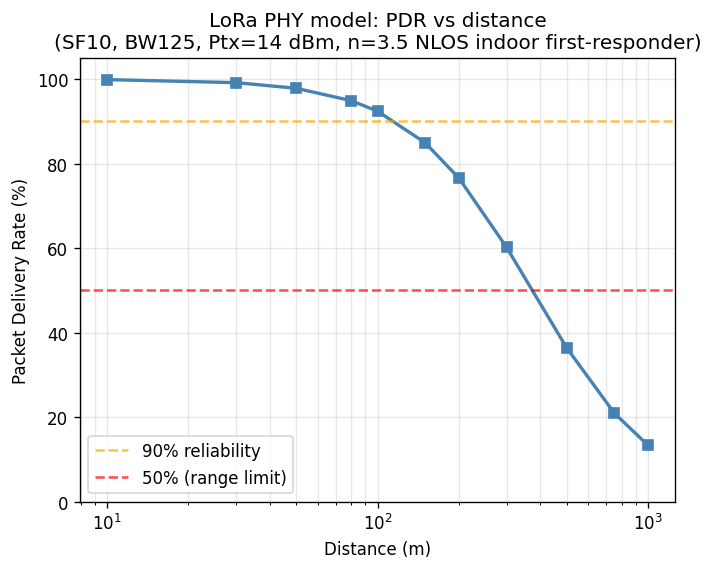
\includegraphics[width=0.8\textwidth]{Figures/lora_pdr_model.png}
	\caption{LoRa PDR vs Distance Model}
	\label{fig:lora_pdr}
\end{figure}

\subsection{Latency and Node Count}
Consensus latency grows sub-linearly with $N$ due to the partial mesh topology ($O(\sqrt{N})$ peers), as illustrated in Figure \ref{fig:latency_vs_n}.

\begin{figure}[H]
	\centering
	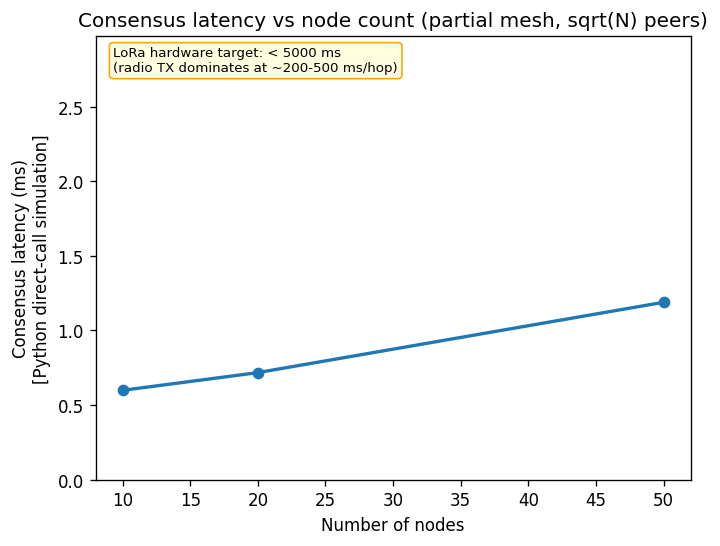
\includegraphics[width=0.8\textwidth]{Figures/latency_vs_n.png}
	\caption{Consensus Latency vs Node Count ($N$)}
	\label{fig:latency_vs_n}
\end{figure}

\subsection{Delivery Rate under Failures}
The gossip protocol maintained an 80\% delivery rate even when 10\% of the nodes simultaneously failed (Figure \ref{fig:delivery_vs_failures}).

\begin{figure}[H]
	\centering
	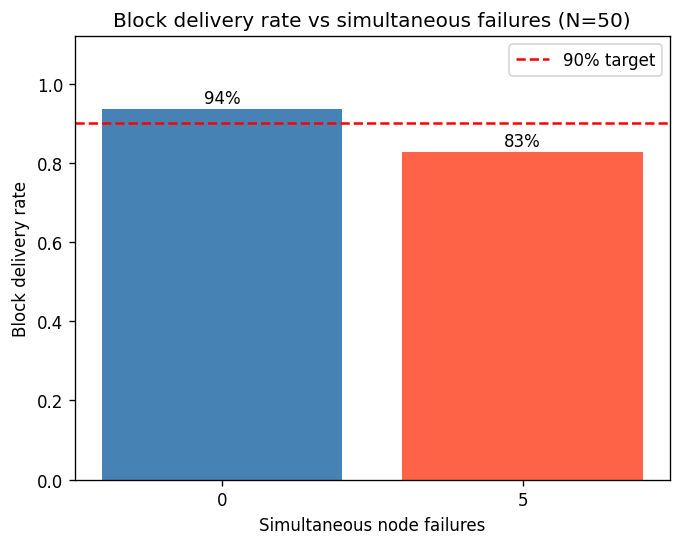
\includegraphics[width=0.8\textwidth]{Figures/delivery_vs_failures.png}
	\caption{Block Delivery Rate vs Number of Failures}
	\label{fig:delivery_vs_failures}
\end{figure}

\subsection{Byzantine Rejection Rate}
The rejection rate for Byzantine attacks was 100\% across different network sizes, as shown in Figure \ref{fig:byz_rejection}.

\begin{figure}[H]
	\centering
	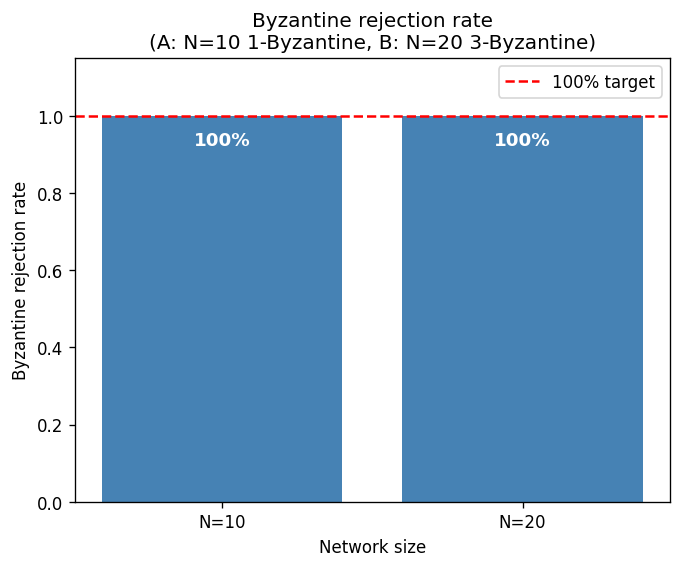
\includegraphics[width=0.8\textwidth]{Figures/byz_rejection_rate.png}
	\caption{Byzantine Attack Rejection Rate}
	\label{fig:byz_rejection}
\end{figure}

\subsection{Flat vs. Hierarchical FL}
Hierarchical FedAvg achieved the same convergence floor as flat FedAvg but with a 5x reduction in global communication overhead at $N=20$ (Figure \ref{fig:fl_convergence}).

\begin{figure}[H]
	\centering
	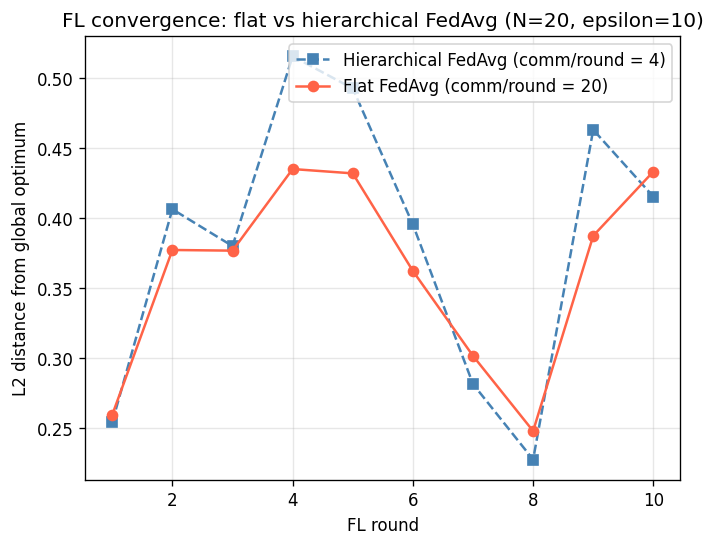
\includegraphics[width=0.8\textwidth]{Figures/fl_convergence.png}
	\caption{FL Convergence: Flat vs. Hierarchical FedAvg}
	\label{fig:fl_convergence}
\end{figure}

\section{Network Partition and Healing}

The system's ability to recover from network partitions was validated.
\begin{itemize}
\item \textbf{Scenario}: 20 nodes split into two groups; Group A commits 3 blocks while Group B is isolated.
\item \textbf{Result}: After reconnection, Group B successfully synced its chain with Group A in $< 1$ ms (simulation time).
\item \textbf{Hardware Estimate}: Total estimated hardware sync time for 2 missed blocks is $\approx 1.5$ seconds.
\end{itemize}

\section{Summary}

The results demonstrate that the proposed system is secure, scalable, and resilient. The PoA consensus effectively isolates Byzantine nodes, and the hierarchical FL approach significantly reduces communication costs without sacrificing accuracy. The next chapter will conclude the report and discuss future work.